 
 
\documentclass[12pt]{article}

\usepackage{fullpage}
\usepackage{multicol,multirow}
\usepackage{tabularx}
\usepackage{ulem}
\usepackage[utf8]{inputenc}
\usepackage[russian]{babel}
\usepackage{graphicx}
\usepackage{float}

\begin{document}

\section*{Лабораторная работа №\,4 по курсу дискрeтного анализа: сортировка за линейное время}

Выполнил студент группы 08-208 МАИ \textit{Куликов Алексей}.

\subsection*{Условие}

Кратко описывается задача: 
\begin{enumerate}
\item Необходимо реализовать один из стандартных алгоритмов поиска образцов для указанного
алфавита.
\item В качестве конкретного задания предлагается поиск одного образца основанный на построении Z-блоков. Алфавит --  слова не более 16 знаков латинского алфавита (регистронезависимые)(Вариант 4-1).
\end{enumerate}

\subsection*{Метод решения}
Весь текст для поиска сохранять нельзя т.к. он потенциально может быть достаточно большим. Поэтому будем сохранять только некоторое <<окно>> длиной в 2 образца (+ сам образец и символ-сентинел. Это даст оценку по памяти в O(M), где M -- длина образца, а не O(N), где N -- длина текста. Чаще всего длина образца много меньше длины текста, поэтому это позволит нам существенно сократить объем требуемой памяти для обработки. Структура будет следующей: [P\$T1T2]. Здесь P -- паттерн, \$ -- символ-сентинел, не входящий в алфавит, T1 и T2 -- ккакие-то кусочки из текста идущие по порядку.

Но теперь придется искать вхождения <<на лету>>. Для того чтобы их не пропускать будем на каждой итерации сдвигать окно на длину образца и вычислять Z-функцию для окна, начиная с символа стоящего после сентинела. Там, где значение Z-функции будет равна длине образца, и есть вхождение. Вывод значений будем осуществлять со второго символа после сентинела. Это позволит дважды не выводить координаты вхождения, если оно попало точь-в-точь в T2.

Координаты считанных символов так же будем хранить в векторе пар <строка, слово> и выводить соответствущие значения на экран, если есть вхождение.

\subsection*{Описание программы}

Программа состоит из одного единственного файла. В ней содержится основная функция и две подсобные: функция рассчитывающая Z-функцию для вектора слов и фунция приведения строки к верхнему регисту. Все остальное происходит в функции main.

\subsection*{Дневник отладки}

\begin{enumerate}
    \item 28.11 16:00. Ответы совсем не совпадают с эталонными для первых тестов. По всей видимсоти, не правильно понял формат входных данных.\\
    РЕШЕНИЕ: Переделал систему ввода.
    \item 28.11 17:00. На одном из тестов неправильно вычисляется Z-функция\\
    РЕШЕНИЕ: Перечитал описание алгоритма. Проблема была в том, что ...
    \item 30.11 11:00. Не проходит 14-й тест. Программа получает сигнал SIGABRT.\\
    РЕШЕНИЕ: Ищем причину ошибки. По всей видимости Это происходит из-за необработанного исключения \verb|bad_alloc| при попытке выделения памяти, когда больше выделить не дает ограничение на чекере. Будем сокращать потребляемую память.
    \item 30.11 13:00. Объем памяти достаточно сократить не получается.\\
    РЕШЕНИЕ: Долгие раздумья. Пришел к идее решения, описанной выше.
    \item 13.12 16:00. Никак не проходится 17-й тест \\
    РЕШЕНИЕ: Пишем генератор тестов. Гоняем тесты (много больших правильных полных тестов с правильными сгенерированными на них ответами).
    \item 18.12 20:00. Ошибки не нашлось. \\
    РЕШЕНИЕ: Принято решение обратиться к преподавателю и спросить про этот тест. Оказывается в некоторых строках в конце находятся trailling-space'ы. Оходим эту проблему фильтрацией ввода (<<проглатываем>> пробелы при помощи \verb|std::ws|).
    
\end{enumerate}

\subsection*{Тест производительности}

\begin{center}
    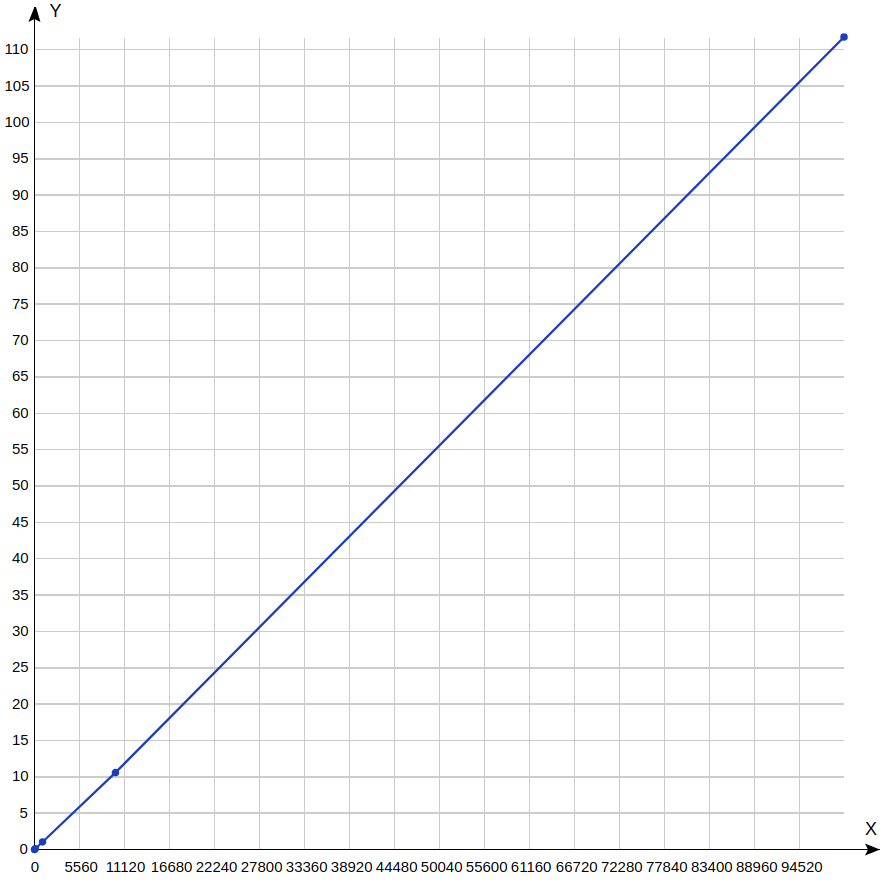
\includegraphics[width=\linewidth]{graph.png}
\end{center}

\begin{table}[H]
\caption{Скорость работы программы}
\label{tabular:timesandtenses}
\begin{center}
\begin{tabular}{|l|c|}
\hline
\textbf{Количество вхождений (шт.)} & \textbf{Время работы (с.)} \\
\hline
10 & 0,017 \\
\hline
100 & 0,111 \\
\hline
1000 & 1,014 \\
\hline
10000 & 10,581 \\
\hline
100000 & 111,743 \\
\hline
\end{tabular}
\end{center}
\end{table}

\subsection*{Недочёты}
Алгоритм работает корректно даже для больших объемов данных (проверено, еогда гонялись тесты). Вероятно эту идею можно улучшить на основе структуры рассматриваемой строки и сдвигать на разные длины. Так же хочется отметить, что лаконичный код для порционного считывания данных из потока. Это, пожалуй единственное, чем я остался недоволен.

\subsection*{Выводы}

Данный алгоритм, вероятно, может применяться непосредственно по назначению в тех случаях, когда нет времени разбираться с более сложными, но лучшими алгоритмами.
В целом, алгоритм имеет линейную зависимость времени выполнения, поэтому это явно не худший вариант, и его вполне можно применить в решении задач, где скорость не очень критичка, а критична именно его способность поиска <<на лету>> без сохранения большого объема данных.

Идея, кажется, довольно простая, особенно когда уже реализована. Сложность программирования алгоритма скорее заключалась в понимании, как вычисляется Z-функция за линейное время, ну и в первых поползновениях к этой идее на листе бумаги.

\end{document}
